\documentclass[usletter]{article}
\usepackage{graphicx}
\usepackage{amsfonts}
\usepackage{amsthm}
\usepackage{amsmath}
\usepackage{amssymb}
\usepackage{scribe}
\usepackage[margin=1.5in]{geometry}

\begin{document}


\makeheader{John Bender}               % your name
           {January 6, 2014}           % lecture date
           {1}                         % lecture number
           {Deterministic Computation} % lecture title

\noindent

The first lecture was an introduction to deterministic computation by way of a review and formalization of the Turing machine, its properties, and how those properties affect execution time. In addition we discussed the impact of restricting a Turing machine with an arbitrary alphabet to a binary alphabet and also restricting one with bidirectional, infinite tapes to unidirectional infinite tapes. Along the way we also saw key definitions and concepts related to understanding computation using Turing machines.

Before reviewing the content a brief summary of notation:

\begin{itemize}
  \item $\{0,1\}^n$ represents an arbitrary string of length $n$ composed of elements from the set $\{0,1\}$.
  \item $\{0,1\}^*$ represents an arbitrary string of arbitrary length composed of elements from the set $\{0,1\}$.
  \item When referring to an alphabet for a Turing machine the inclusion of $\rhd$ and $\Box$ is often implicit.
  \item A function $f : X \rightarrow Y$ ``has the type'' $X \rightarrow Y$ when it takes an argument of type $X$ and returns an argument of type $Y$.
  \item A function $f : M \times N \rightarrow X$ can be viewed as accepting a pair such as $(x, y)$ where $x : M$ and $y : N$ and returning something of type $X$.
  \item Terms emphasized with \textit{italics} are definitional terms of particular importance to the material.
\end{itemize}

\section{Turing machines} \label{sec:turing-machines}

First, at a high level, we examine the components needed for a Turing machine to perform computation in order to facilitate a basic understanding of their operation.

\begin{enumerate}
  \item A finite but arbitrarily large set of \textit{tapes},  where the cardinality of the set is often denoted by $k$, and each tape has an infinite number of discrete \textit{cells}.
  \item $k$ \textit{heads} that read and write to a single cell on each tape and also handle the movement between cells.
  \item A finite \textit{alphabet}, $\Gamma$, that contains the symbols each head will write to and read from the tapes.
  \item A register or registers that stores the current \textit{state} of the Turing machine from the finite set of possible states $Q$.
  \item A \textit{transition function}, $\delta$, that maps from the symbols in the $k$ cells currently under each head and the current state to symbols for the same cells, a movement (or lack thereof) for each head, and a new state.
\end{enumerate}

\begin{figure}
\begin{center}
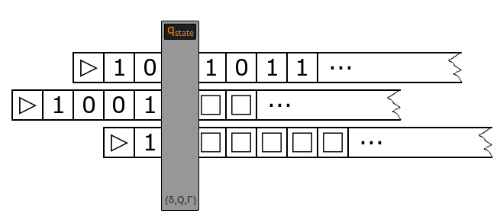
\includegraphics[width=1\textwidth]{lectures/graphics/turing-machine}
\end{center}
\caption{A Turing machine}
\label{fig:turing-machine}
\end{figure}

More formally we have the following definition for the Turing machine itself (everything but the tapes).

\begin{definition}
  \textbf{Turing Machine}. A Turing machine is a tuple $(\Gamma, Q, \delta)$ with the following properties.
  \begin{enumerate}
    \item $\Gamma$ is a finite but arbitrary set, referred to as an \textit{alphabet}, that must contain at least $\rhd, \Box$ and two other distinct, unique symbols.
    \item $Q$ is a set of finite but arbitrary set of \textit{states} that must contain at least $\textsf{START}$ and $\textsf{HALTED}$.
    \item $\delta$ is a function of the type $Q \times \Gamma^{k} \rightarrow Q \times \Gamma^{k-1} \times \{\leftarrow, \cdot, \rightarrow\}^k$, referred to as the \textit{transition function} where $k$ is the finite but arbitrarily large number of tapes that the machine uses.
  \end{enumerate}
\end{definition}


Assuming the above description and definition, a single \textit{step} of a Turing machine's execution proceeds by, first observing the current cell values and current state value, and then writing the new symbols, new state and moving each tape based on the result from $\delta$. The physical metaphor is represented in Figure \ref{fig:turing-machine} but a more detailed description of each component may be helpful.

Tapes normally start as far to the left as possible. That is, most Turing machines consist of tapes that only extend to the right infinitely. As we'll see later, even those that extend in both directions can be \textit{reduced} to a Turing machine that only extends infinitely in one direction. Also, one of the tapes is the \textit{input tape} and the head for that tape is \textit{read-only}. That is, the transition function can never tell the head for the input tape to write or similarly must always write the same symbol back. All other tapes start blank save for the start symbol at the beginning.

The heads for each tape are responsible for reading values as input to the transition function, $\delta$, and writing the output from $\delta$ to the $k-1$ \textit{read-write} tapes. They are also responsible for moving the tape left one cell, right one cell, or not at all depending on the output of $\delta$. Each of those movement operations is represented by $\leftarrow$, $\rightarrow$, and $\cdot$. Finally, When a head attempts to move the tape right at the tape's left-most extent it will simply stay put.

The alphabet $\Gamma$ must, at a minimum, contain both the start symbol, $\rhd$, the blank symbol $\Box$ and at least two more symbols to perform any computation. $\rhd$ is used to signal to the transition function, $\delta$, when a given head is at the left-most extent of its tape. The second is normally used to signify the end of other symbols on a given tape. Most often $\Gamma$ is simply the set $\{\rhd, \Box, 0, 1\}$. Otherwise the alphabet can contain a finite number of arbitrary symbols, but as we'll discuss later it is possible to ``encode'' all other alphabets using the simple one.

The state register assumes values from a the finite set $Q$ that must contain the states \textsf{START} and \textsf{HALT} but is otherwise arbitrary. Some Turing machines have many registers but once again these can be encoded for use with a single register by taking the cartesian product of each set of possible states for the individual registers \cite{textbook}.

Finally, examining the type of $\delta$, namely $Q \times \Gamma^{k} \rightarrow Q \times \Gamma^{k-1} \times \{\leftarrow, \cdot, \rightarrow\} ^k$, you can see that it takes a single state from $Q$ and $k$ symbols from $\Gamma$, corresponding to the cells of the $k$ tapes currently under each head, as input and produces a new state from $Q$, $k-1$ new symbols for the same cells (the input tape is read-only), and $k$ movements for each head to perform.

\section{Palindrome turing machine}

Now we examine an example Turing machine that determines whether a given input is a palindrome to establish further intuition about how a Turing machine is constructed. First we define a palindrome using binary strings.

\begin{definition}
  \textbf{Palindrome}. $x \in \{0, 1\}^n$ is a palindrome if, when taken as a sequence, $\langle x_1,x_2,\ldots,x_n \rangle = \langle x_n,\ldots,x_2,x_1\rangle$
\end{definition}

With that in mind we can sketch the construction of a Turing machine to check an arbitrary but finite binary string to see if it is a palindrome.

\begin{enumerate}
  \item It will have three tapes: the input tape, output tape and one work tape. That is $k = 3$
  \item It will use the binary alphabet, $\Gamma = \{\rhd, \Box, 0, 1\}$.
  \item It will have five states, $Q = \{ \textsf{START}, \textsf{HALT}, \textsf{COPY}, \textsf{LEFT}, \textsf{TEST}\} $.
  \item It will have a transition function $\delta$ that conforms to the following sequence of steps:
    \begin{enumerate}
      \item Copy all symbols from the input tape to the same cells on the work tape, until both heads for these tapes are at the end of the input.
      \item Return the head of the work tape to its left most cell.
      \item Begin comparing each cell of the work tape and the input tape, proceeding right and left respectively.
      \item If at any point the value of the cell under either head is different output 0 to the output tape and halt.
      \item If input tape reaches $\rhd$ then output 1 to the output tape and halt.
    \end{enumerate}
\end{enumerate}

To illustrate further we define $\delta$ as a mapping in tabular form.

\vspace{0.5cm}

\begin{tabular}{ | a | b | c | d | e | f | g | h | i | j | k | }
    \hline
    \multicolumn{4}{|i|}{Input} & \multicolumn{6}{|i|}{Ouput}\\
    \hline
    \multicolumn{3}{|i|}{Tapes}& \multicolumn{1}{|i|}{State} &
      \multicolumn{2}{|i|}{Tapes} & \multicolumn{1}{|i|}{State} & \multicolumn{3}{|i|}{Movement}\\
    \hline
    in$_{in}$ & wrk$_{in}$ & out$_{in}$ &  sta$_{in}$ &
      wrk$_{out}$ & out$_{out}$ & sta$_{out}$ & in$_{mv}$ & wrk$_{mv}$ & out$_{mv}$  \\
    \hline

    \rhd & \rhd & \rhd & \textsf{START} &
      \rhd & \rhd & \textsf{COPY} & \rightarrow & \rightarrow & \rightarrow \\
    \hline

    0 & \Box & $\Box$ & \textsf{COPY} &
      0 & \Box & \textsf{COPY} & \rightarrow & \rightarrow & \cdot \\
    \hline

    1 & $\Box$ & $\Box$ & \textsf{COPY} &
      1 & $\Box$ & \textsf{COPY} & $\rightarrow$ & $\rightarrow$ & $\cdot$ \\
    \hline

    $\Box$ & $\Box$ & $\Box$ & \textsf{COPY} &
      $\Box$ & $\Box$ & \textsf{LEFT} & $\cdot$ & $\leftarrow$ & $\cdot$ \\
    \hline

    $\Box$ & 0 & $\Box$ & \textsf{LEFT} &
      0 & $\Box$ & \textsf{LEFT} & $\cdot$ & $\leftarrow$ & $\cdot$ \\
    \hline

    $\Box$ & 1 & $\Box$ & \textsf{LEFT} &
      1 & $\Box$ & \textsf{LEFT} & $\cdot$ & $\leftarrow$ & $\cdot$ \\
    \hline

    $\Box$ & $\rhd$ & $\Box$ & \textsf{LEFT} &
      $\rhd$ & $\Box$ & \textsf{TEST} & $\leftarrow$ & $\rightarrow$ & $\cdot$ \\
    \hline

    1 & 1 & $\Box$ & \textsf{TEST} &
      1 & $\Box$ & \textsf{TEST} & $\leftarrow$ & $\rightarrow$ & $\cdot$ \\
    \hline

    0 & 0 & $\Box$ & \textsf{TEST} &
      0 & $\Box$ & \textsf{TEST} & $\leftarrow$ & $\rightarrow$ & $\cdot$ \\
    \hline

    1 & 0 & $\Box$ & \textsf{TEST} &
      0 & 0 & \textsf{HALT} & $\cdot$ & $\cdot$ & $\cdot$ \\
    \hline

    0 & 1 & $\Box$ & \textsf{TEST} &
      1 & 0 & \textsf{HALT} & $\cdot$ & $\cdot$ & $\cdot$ \\
    \hline

    $\rhd$ & $\Box$ & $\Box$ & \textsf{TEST} &
      $\Box$ & 1 & \textsf{HALT} & $\cdot$ & $\cdot$ & $\cdot$ \\
    \hline
  \end{tabular}

\vspace{0.5cm}

As you can see this is a relatively straight forward function, though in most cases enumerating all the steps for a Turing machine that is even slightly more complex would be difficult and time consuming.

\section{Efficiency}

Having thoroughly defined what a Turing machine is we can explore what it means for a Turing machine to complete its task efficiently.

The efficiency of a Turing machine is captured as a function of type $\mathbb{N} \rightarrow \mathbb{N}$, of the length of inputs to the machine. Intuitively, the speed at which the Turing machine is able to complete its task is most frequently a function of the length of the input. More formally we have the following definition:

\begin{definition}
  \textbf{Efficiency}. A Turing machine computes a function $f:\{0,1\}^* \rightarrow \{0,1\}^*$ in time $T(n)$ if, when started with any string $x \in \{0,1\}^*$, the Turing machine halts within $T(|x|)$ steps with $f(x)$ on the output tape.
\end{definition}

\begin{example}
  \textbf{Palindrome}. It's clear that in this case, $T(n) = 3n$. The contents of the input tape must be copied in full to the work tape ($n$ steps), the work tape must be traversed to its starting point ($n$ steps), and then both the input tape and the work tape must be assessed simultaneously ($n$ steps).
\end{example}

Additionally we have the notion of a \textit{language} which is any set of strings composed from any finite length alphabet (though we consider only the binary alphabet here).

\begin{definition}
  \textbf{Language}. A language is any subset of $\{0, 1\}^*$ where $\{0, 1\}$ is the alphabet under consideration.
\end{definition}

\begin{example}
  \textbf{Even Length Strings}. All strings $x$ where $x \in \{0, 1\}^*$ and $|x| \bmod 2 = 0$.
\end{example}

\begin{example}
  \textbf{Strings Starting with 0}. All strings $x$ where $x \in \{0, 1\}^*$ and $x_1 = 0$ .
\end{example}

Of primary concern is the ability to find a Turing machine that \textit{decides} a language. That is, for an arbitrary string $x$ a Turing machine decides a language $L$ if it can verify membership of $x$ in $L$.

\begin{definition}
  \textbf{Deciding a Language}. A Turing machine $M$ decides a language, $L$,  where $ L \subseteq \{0,1\}^*$, if $M$ computes the function $f_L : \{0, 1\}^* \rightarrow \{0,1\}$ where:
  \begin{equation*}
    f_L(x) =
    \begin{cases}
      1\ \text{if}\ x \in L \\
      0\ \text{otherwise}
    \end{cases}
  \end{equation*}
\end{definition}

To accompany the notions of languages and deciding a language, there are classes of languages to which a one might belong based on the efficiency of its deciding Turing machine. For example, if some language $L$ has a \textit{deterministic} Turing machine (from whence the \textbf{D} is derived) that decides $L$ in some time $T(n)$ then it belongs to the family \textbf{DTIME}$(T(n))$ \cite{textbook}.

\begin{definition}
  \textbf{DTIME}$(T(n))$ is the family of all languages $L$ decideable in the time $C(T(n))$ for some constant $C$ where $C > 0$.
\end{definition}

Finally we have the definition for the class of languages \textbf{P}. Here, \textbf{P} stands for polynomial and this class includes all languages that are decidable by a Turing machine in time $T(n)$ where $T(n)$ is a polynomial function of $n$.

\begin{definition}
  \textbf{P} $= \bigcup\limits_{i=1}^{\infty} \textbf{DTIME}(n^i)$
\end{definition}

It's important to note that while it may appear that the function is exponential due to $i$ taken to $\infty$ it is actually the case that $i$ is fixed when considering a function $T(n)$ for membership in \textbf{P} and therefore the function is polynomial (not super confident here).

\section{Alternate Turing machines}

Here we consider the impact of modifications to different aspects of a Turing machine. In particular we examine the impact of encoding other alphabets to $\{0,1\}$ and the impact of representing bi-directional tapes as ``stacked'' unidirectional tapes. The key intuition we get from examining these transformations is that the we can always consider complexity problems using a binary Turing machine of the form described in Section \ref{sec:turing-machines}.

\begin{theorem}
  If $f : \{0,1\}^* \rightarrow \{0,1\}^*$ is computable in time $T(n)$ with some alphabet $\Gamma$, then $f$ is computable in time $O(log_2(|\Gamma|)T(n))$ with the alphabet $\{\rhd,\Box, 0, 1\}$.
\end{theorem}

Note that in the theorem $O(log_2(|\Gamma|)T(n))$ is equivalent to $O(T(n))$ since $log_2(|\Gamma|)$ is a constant, but it is included for clarity on the slow down incurred by encoding the alphabet $\Gamma$ using the binary alphabet.

\begin{figure}
\begin{center}
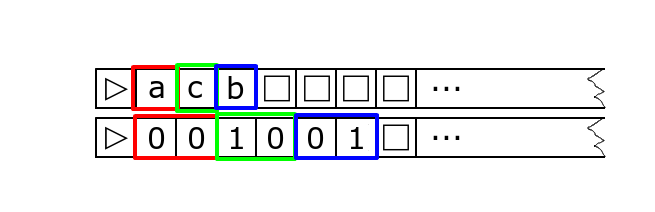
\includegraphics[width=1\textwidth]{lectures/graphics/encoding}
\end{center}
\caption{Unencoded and Encoded Tapes}
\label{fig:encoding}
\end{figure}

To illustrate we have two trivial example tapes in Figure \ref{fig:encoding}. The first uses the alphabet $\{\rhd, \Box, a, b, c\}$ and the second encodes the first using the binary alphabet. A Turing machine using the binary alphabet to simulate a Turing machine using alphabet $\Gamma$ would proceed as follows:

\begin{enumerate}
  \item In place of reading a single symbol from each tape, it must read $log_2(|\Gamma|)$ symbols from each tape.
  \item Each symbol read must be ``remembered'' in the state of the Turing machine until $log_2(|\Gamma|)$ symbols are read from each tape.
  \item The transition function then has enough information to determine what the simulated transition function would output.
  \item The output is then written to $log_2(|\Gamma|)$ cells. Note that after writing the encoded symbol to the current set of cells the head will be at its previous starting position.
  \item Each head may be moved either 0 or $log_2(|\Gamma|)$ cells corresponding to no move and a move to the left or right.
\end{enumerate}

Note that both the $\delta$ and $Q$ for the binary Turing machine help to absorb the complexity of the encoding. That is, $\delta$ must now transition between two general modes, reading and computing and $Q$ must permit the storage of incomplete symbol during the reading.

\begin{figure}
\begin{center}
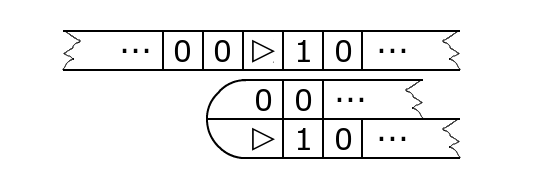
\includegraphics[width=1\textwidth]{lectures/graphics/folded}
\end{center}
\caption{Bidirectional and Folded Tapes}
\label{fig:folded}
\end{figure}


Next we consider the impact of representing infinite bidirectional tapes using a single folded unidirectional tape. In Figure \ref{fig:folded} is one approach to representing a bidirectional tape (top) using a unidirectional tape (bottom) by ``folding'' the tape. Intuitively, the cells of the new tape encode symbols from an alphabet $\Gamma'$ that is the cartesian product of the original alphabet with itself, $\Gamma' = \Gamma \times \Gamma$ and $\delta'$ will account for traversal of the tape past $\rhd$ by registering which side should be considered, Top or Bottom, in the state. That is, $Q' = Q \times \{\text{Top}, \text{Bottom}\}$.

There are a few cases work examining to understand this further:

\begin{itemize}
  \item When the cell under consideration is the physical leftmost, the state includes Top, and the original $\delta$ would move right, the head remains at that cell and instead writes a new state that includes Bottom instead of Top.
  \item Similarly for the bottom leftmost cell when $delta$ would move left the head remains at  that cell and instead writes a new state that includes Top instead of Bottom.
  \item When the current state of the Turing machine includes Top and the movement direction from the original $\delta$ would be \textit{right} the tape must proceed left on the folded tape. That is the Top tape is ``upside-down''.
  \item When the current state of the Turing machine includes Bottom the movement proceeds as normal.
\end{itemize}

\newpage

Finally, we consider the impact on the execution time when folding a tape this way. Given that the only extra complexity exists in $\delta$'s accounting for the Top and Bottom state it's fairly clear that $T'(n) = O(T(n))$.

\begin{theorem}
  If a function $f:\{0,1\}^* \rightarrow \{0,1\}^*$ is computable in time $T(n)$ with bidirectional tapes, then it is computable in time $O(T(n))$ with unidirectional tapes.
\end{theorem}

\begin{proof}
  By the definition of $O(T(n))$ we must argue that, for every $n$ steps of the original bidirectional Turing machine $M$, the unidirectional ``folded'' tape Turing machine $M'$ will take at most $C \cdot n$ steps. Where $C$ is some constant independent of the input length, $|x|$. We use the model from Figure \ref{fig:folded} to argue that $M'$ will take \textit{at most} $n$ steps and therefore $C \le 1$. Consider three cases:

  \begin{description}
    \item[From left of $\rhd$ to left of $\rhd$ on $M$s tape.] Then the cells of $M$s tape correspond to the first symbols of the pairs in $M'$s tape. So, where $M$ would take $n$ steps to traverse left, $M'$ can traverse right $n$ steps. So, $T(n) = T'(n)$.

    \item[From $\rhd$ to right of $\rhd$ on $M$s tape.] Then the cells of $M$s tape correspond to the second symbols of the pairs in $M'$s tape. So, where $M$ would take $n$ steps to traverse right, $M'$ can traverse right $n$ steps. So, $T(n) = T'(n)$.

    \item[From either side of $\rhd$ to the other on $M$s tape.] Now suppose that the head of $M$ is $i$ steps from $\rhd$ and the destination is $j$ steps further from $\rhd$, such that $n = i + j$. Now $M$ must take $n$ steps but $M'$ can ``jump'' from Top to Bottom or vice versa and take only $|i - j|$ steps. So $T(n) \ge T'(n)$. In particular, the best case $i = j$ requires exactly one step for $M'$ to update the state and write the pair back to the same cell and in the worst case $i = 0$  or $j = 0$ so $M'$ requires $n$ steps resulting in $0 < C \le 1$.
  \end{description}

Thus, $C = 1$ for the first two cases $0 < C \le 1$ for the last.
\end{proof}


\newpage

\bibliographystyle{abbrv}
\bibliography{1}

\end{document}
